% Options for packages loaded elsewhere
\PassOptionsToPackage{unicode}{hyperref}
\PassOptionsToPackage{hyphens}{url}
\PassOptionsToPackage{dvipsnames,svgnames,x11names}{xcolor}
%
\documentclass[
  letterpaper,
  DIV=11,
  numbers=noendperiod]{scrartcl}

\usepackage{amsmath,amssymb}
\usepackage{iftex}
\ifPDFTeX
  \usepackage[T1]{fontenc}
  \usepackage[utf8]{inputenc}
  \usepackage{textcomp} % provide euro and other symbols
\else % if luatex or xetex
  \usepackage{unicode-math}
  \defaultfontfeatures{Scale=MatchLowercase}
  \defaultfontfeatures[\rmfamily]{Ligatures=TeX,Scale=1}
\fi
\usepackage{lmodern}
\ifPDFTeX\else  
    % xetex/luatex font selection
\fi
% Use upquote if available, for straight quotes in verbatim environments
\IfFileExists{upquote.sty}{\usepackage{upquote}}{}
\IfFileExists{microtype.sty}{% use microtype if available
  \usepackage[]{microtype}
  \UseMicrotypeSet[protrusion]{basicmath} % disable protrusion for tt fonts
}{}
\makeatletter
\@ifundefined{KOMAClassName}{% if non-KOMA class
  \IfFileExists{parskip.sty}{%
    \usepackage{parskip}
  }{% else
    \setlength{\parindent}{0pt}
    \setlength{\parskip}{6pt plus 2pt minus 1pt}}
}{% if KOMA class
  \KOMAoptions{parskip=half}}
\makeatother
\usepackage{xcolor}
\setlength{\emergencystretch}{3em} % prevent overfull lines
\setcounter{secnumdepth}{-\maxdimen} % remove section numbering
% Make \paragraph and \subparagraph free-standing
\ifx\paragraph\undefined\else
  \let\oldparagraph\paragraph
  \renewcommand{\paragraph}[1]{\oldparagraph{#1}\mbox{}}
\fi
\ifx\subparagraph\undefined\else
  \let\oldsubparagraph\subparagraph
  \renewcommand{\subparagraph}[1]{\oldsubparagraph{#1}\mbox{}}
\fi

\usepackage{color}
\usepackage{fancyvrb}
\newcommand{\VerbBar}{|}
\newcommand{\VERB}{\Verb[commandchars=\\\{\}]}
\DefineVerbatimEnvironment{Highlighting}{Verbatim}{commandchars=\\\{\}}
% Add ',fontsize=\small' for more characters per line
\usepackage{framed}
\definecolor{shadecolor}{RGB}{241,243,245}
\newenvironment{Shaded}{\begin{snugshade}}{\end{snugshade}}
\newcommand{\AlertTok}[1]{\textcolor[rgb]{0.68,0.00,0.00}{#1}}
\newcommand{\AnnotationTok}[1]{\textcolor[rgb]{0.37,0.37,0.37}{#1}}
\newcommand{\AttributeTok}[1]{\textcolor[rgb]{0.40,0.45,0.13}{#1}}
\newcommand{\BaseNTok}[1]{\textcolor[rgb]{0.68,0.00,0.00}{#1}}
\newcommand{\BuiltInTok}[1]{\textcolor[rgb]{0.00,0.23,0.31}{#1}}
\newcommand{\CharTok}[1]{\textcolor[rgb]{0.13,0.47,0.30}{#1}}
\newcommand{\CommentTok}[1]{\textcolor[rgb]{0.37,0.37,0.37}{#1}}
\newcommand{\CommentVarTok}[1]{\textcolor[rgb]{0.37,0.37,0.37}{\textit{#1}}}
\newcommand{\ConstantTok}[1]{\textcolor[rgb]{0.56,0.35,0.01}{#1}}
\newcommand{\ControlFlowTok}[1]{\textcolor[rgb]{0.00,0.23,0.31}{#1}}
\newcommand{\DataTypeTok}[1]{\textcolor[rgb]{0.68,0.00,0.00}{#1}}
\newcommand{\DecValTok}[1]{\textcolor[rgb]{0.68,0.00,0.00}{#1}}
\newcommand{\DocumentationTok}[1]{\textcolor[rgb]{0.37,0.37,0.37}{\textit{#1}}}
\newcommand{\ErrorTok}[1]{\textcolor[rgb]{0.68,0.00,0.00}{#1}}
\newcommand{\ExtensionTok}[1]{\textcolor[rgb]{0.00,0.23,0.31}{#1}}
\newcommand{\FloatTok}[1]{\textcolor[rgb]{0.68,0.00,0.00}{#1}}
\newcommand{\FunctionTok}[1]{\textcolor[rgb]{0.28,0.35,0.67}{#1}}
\newcommand{\ImportTok}[1]{\textcolor[rgb]{0.00,0.46,0.62}{#1}}
\newcommand{\InformationTok}[1]{\textcolor[rgb]{0.37,0.37,0.37}{#1}}
\newcommand{\KeywordTok}[1]{\textcolor[rgb]{0.00,0.23,0.31}{#1}}
\newcommand{\NormalTok}[1]{\textcolor[rgb]{0.00,0.23,0.31}{#1}}
\newcommand{\OperatorTok}[1]{\textcolor[rgb]{0.37,0.37,0.37}{#1}}
\newcommand{\OtherTok}[1]{\textcolor[rgb]{0.00,0.23,0.31}{#1}}
\newcommand{\PreprocessorTok}[1]{\textcolor[rgb]{0.68,0.00,0.00}{#1}}
\newcommand{\RegionMarkerTok}[1]{\textcolor[rgb]{0.00,0.23,0.31}{#1}}
\newcommand{\SpecialCharTok}[1]{\textcolor[rgb]{0.37,0.37,0.37}{#1}}
\newcommand{\SpecialStringTok}[1]{\textcolor[rgb]{0.13,0.47,0.30}{#1}}
\newcommand{\StringTok}[1]{\textcolor[rgb]{0.13,0.47,0.30}{#1}}
\newcommand{\VariableTok}[1]{\textcolor[rgb]{0.07,0.07,0.07}{#1}}
\newcommand{\VerbatimStringTok}[1]{\textcolor[rgb]{0.13,0.47,0.30}{#1}}
\newcommand{\WarningTok}[1]{\textcolor[rgb]{0.37,0.37,0.37}{\textit{#1}}}

\providecommand{\tightlist}{%
  \setlength{\itemsep}{0pt}\setlength{\parskip}{0pt}}\usepackage{longtable,booktabs,array}
\usepackage{calc} % for calculating minipage widths
% Correct order of tables after \paragraph or \subparagraph
\usepackage{etoolbox}
\makeatletter
\patchcmd\longtable{\par}{\if@noskipsec\mbox{}\fi\par}{}{}
\makeatother
% Allow footnotes in longtable head/foot
\IfFileExists{footnotehyper.sty}{\usepackage{footnotehyper}}{\usepackage{footnote}}
\makesavenoteenv{longtable}
\usepackage{graphicx}
\makeatletter
\def\maxwidth{\ifdim\Gin@nat@width>\linewidth\linewidth\else\Gin@nat@width\fi}
\def\maxheight{\ifdim\Gin@nat@height>\textheight\textheight\else\Gin@nat@height\fi}
\makeatother
% Scale images if necessary, so that they will not overflow the page
% margins by default, and it is still possible to overwrite the defaults
% using explicit options in \includegraphics[width, height, ...]{}
\setkeys{Gin}{width=\maxwidth,height=\maxheight,keepaspectratio}
% Set default figure placement to htbp
\makeatletter
\def\fps@figure{htbp}
\makeatother

\KOMAoption{captions}{tableheading}
\makeatletter
\makeatother
\makeatletter
\makeatother
\makeatletter
\@ifpackageloaded{caption}{}{\usepackage{caption}}
\AtBeginDocument{%
\ifdefined\contentsname
  \renewcommand*\contentsname{Table of contents}
\else
  \newcommand\contentsname{Table of contents}
\fi
\ifdefined\listfigurename
  \renewcommand*\listfigurename{List of Figures}
\else
  \newcommand\listfigurename{List of Figures}
\fi
\ifdefined\listtablename
  \renewcommand*\listtablename{List of Tables}
\else
  \newcommand\listtablename{List of Tables}
\fi
\ifdefined\figurename
  \renewcommand*\figurename{Figure}
\else
  \newcommand\figurename{Figure}
\fi
\ifdefined\tablename
  \renewcommand*\tablename{Table}
\else
  \newcommand\tablename{Table}
\fi
}
\@ifpackageloaded{float}{}{\usepackage{float}}
\floatstyle{ruled}
\@ifundefined{c@chapter}{\newfloat{codelisting}{h}{lop}}{\newfloat{codelisting}{h}{lop}[chapter]}
\floatname{codelisting}{Listing}
\newcommand*\listoflistings{\listof{codelisting}{List of Listings}}
\makeatother
\makeatletter
\@ifpackageloaded{caption}{}{\usepackage{caption}}
\@ifpackageloaded{subcaption}{}{\usepackage{subcaption}}
\makeatother
\makeatletter
\@ifpackageloaded{tcolorbox}{}{\usepackage[skins,breakable]{tcolorbox}}
\makeatother
\makeatletter
\@ifundefined{shadecolor}{\definecolor{shadecolor}{rgb}{.97, .97, .97}}
\makeatother
\makeatletter
\makeatother
\makeatletter
\makeatother
\ifLuaTeX
  \usepackage{selnolig}  % disable illegal ligatures
\fi
\IfFileExists{bookmark.sty}{\usepackage{bookmark}}{\usepackage{hyperref}}
\IfFileExists{xurl.sty}{\usepackage{xurl}}{} % add URL line breaks if available
\urlstyle{same} % disable monospaced font for URLs
\hypersetup{
  pdftitle={2.3 Visualisierung mit Grafiken},
  colorlinks=true,
  linkcolor={blue},
  filecolor={Maroon},
  citecolor={Blue},
  urlcolor={Blue},
  pdfcreator={LaTeX via pandoc}}

\title{2.3 Visualisierung mit Grafiken}
\author{}
\date{}

\begin{document}
\maketitle
\ifdefined\Shaded\renewenvironment{Shaded}{\begin{tcolorbox}[frame hidden, sharp corners, borderline west={3pt}{0pt}{shadecolor}, interior hidden, enhanced, breakable, boxrule=0pt]}{\end{tcolorbox}}\fi

\hypertarget{grundlagen}{%
\subsection{Grundlagen}\label{grundlagen}}

Um uns einen Überblick über die Daten zu verschaffen und einfacher
Zusammenhänge zwischen Variablen zu erhalten, ist es oft sinnvoll,
Diagramme zu erstellen. R bietet dafür zahlreiche Möglichkeiten, die
sehr flexibel genutzt werden können.

In dieser Einheit werden wir mit dem Datensatz \texttt{m111survey} aus
dem \texttt{tigerstats}-Paket die Grundlagen für eine solche
Visualisierung erarbeiten. Dieser Datensatz ist das Ergebnis einer
Umfrage unter 71 Studierenden des Georgetown College in Kentucky.

Zunächst laden wir diesen Datensatz in unsere Umgebung.

\begin{Shaded}
\begin{Highlighting}[]
\CommentTok{\# install.packages("tigerstats")}
\end{Highlighting}
\end{Shaded}

\begin{Shaded}
\begin{Highlighting}[]
\FunctionTok{library}\NormalTok{(tidyverse)}
\FunctionTok{library}\NormalTok{(tigerstats)}
\end{Highlighting}
\end{Shaded}

Mithilfe von \texttt{?m111survey} können wir uns ansehen, welche
Bedeutung die Variablen haben. Man könnte zum Beispiel annehmen, dass
Studenten mit niedrigerem Notendurchschnitt eher dazu neigen, schnell zu
fahren. Veranschaulichen wir diesen Zusammenhang in einem Diagramm:

\begin{Shaded}
\begin{Highlighting}[]
\NormalTok{m111survey }\SpecialCharTok{\%\textgreater{}\%} 
  \FunctionTok{ggplot}\NormalTok{(}\FunctionTok{aes}\NormalTok{(}\AttributeTok{x =}\NormalTok{ GPA, }\AttributeTok{y =}\NormalTok{ fastest)) }\SpecialCharTok{+}
  \FunctionTok{geom\_point}\NormalTok{()}
\end{Highlighting}
\end{Shaded}

\begin{verbatim}
Warning: Removed 1 rows containing missing values (`geom_point()`).
\end{verbatim}

\begin{figure}[H]

{\centering 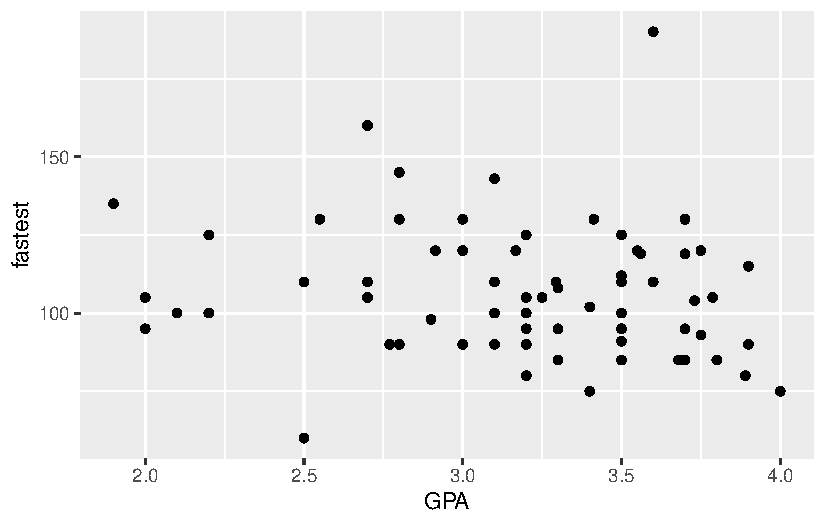
\includegraphics{05-visualisierung_files/figure-pdf/unnamed-chunk-3-1.pdf}

}

\end{figure}

Dieses Diagramm ist ein sogenannter \emph{Scatterplot} bzw. ein
Streudiagramm. Der Aufbau eines solchen Diagramms in R ist wie folgt:

\begin{Shaded}
\begin{Highlighting}[]
\NormalTok{datensatz }\SpecialCharTok{\%\textgreater{}\%} 
  \CommentTok{\# Legt den "Rahmen" und die Achsen fest}
  \FunctionTok{ggplot}\NormalTok{(}\FunctionTok{aes}\NormalTok{(}\AttributeTok{x =}\NormalTok{ x}\SpecialCharTok{{-}}\NormalTok{Achsen}\SpecialCharTok{{-}}\NormalTok{Variable, }\AttributeTok{y =}\NormalTok{ y}\SpecialCharTok{{-}}\NormalTok{Achsen}\SpecialCharTok{{-}}\NormalTok{Variable)) }\SpecialCharTok{+}
\NormalTok{  geom\_... }\SpecialCharTok{+} \CommentTok{\# Das sogenannte "Layer", z.B. Punkte, Linien, Formen, ...}
\NormalTok{  ... }\CommentTok{\# Man kann mehrere Layer übereinander legen.}
\end{Highlighting}
\end{Shaded}

Man könnte denken, dass diese Annahme tatsächlich stimmt. Legen wir mal
eine ``Ausgleichsgerade'' durch die Punkte:

\begin{Shaded}
\begin{Highlighting}[]
\NormalTok{m111survey }\SpecialCharTok{\%\textgreater{}\%} 
  \FunctionTok{ggplot}\NormalTok{(}\FunctionTok{aes}\NormalTok{(}\AttributeTok{x =}\NormalTok{ GPA, }\AttributeTok{y =}\NormalTok{ fastest)) }\SpecialCharTok{+}
  \FunctionTok{geom\_point}\NormalTok{() }\SpecialCharTok{+}
  \FunctionTok{geom\_smooth}\NormalTok{(}\AttributeTok{method =} \StringTok{"lm"}\NormalTok{) }\CommentTok{\# lm steht für "Linear Model"}
\end{Highlighting}
\end{Shaded}

\begin{verbatim}
`geom_smooth()` using formula = 'y ~ x'
\end{verbatim}

\begin{verbatim}
Warning: Removed 1 rows containing non-finite values (`stat_smooth()`).
\end{verbatim}

\begin{verbatim}
Warning: Removed 1 rows containing missing values (`geom_point()`).
\end{verbatim}

\begin{figure}[H]

{\centering 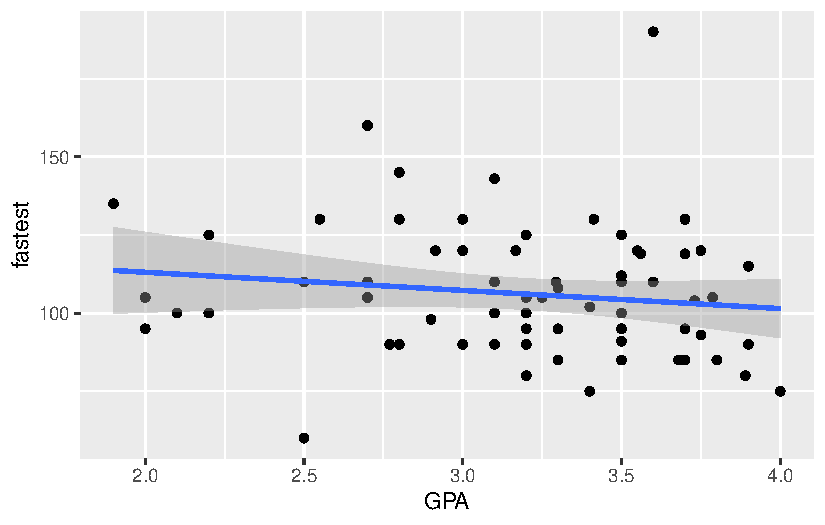
\includegraphics{05-visualisierung_files/figure-pdf/unnamed-chunk-5-1.pdf}

}

\end{figure}

Der graue Balken in diesem Diagramm beschreibt im Grunde die
Unsicherheit in unserem Modell. Wir sehen, dass er so breit ist, dass
die Enden sich jeweils überlappen. Daher können wir nicht darauf
schließen, dass der Notenschnitt einen Einfluss auf die höchste je
gefahrene Geschwindigkeit hat.

Wir können aber mehr aus den Daten holen. Schauen wir uns zum Beispiel
an, wie Frauen im Vergleich zu Männern in der Umfrage antworten:

\begin{Shaded}
\begin{Highlighting}[]
\NormalTok{m111survey }\SpecialCharTok{\%\textgreater{}\%} 
  \FunctionTok{ggplot}\NormalTok{(}\FunctionTok{aes}\NormalTok{(}\AttributeTok{x =}\NormalTok{ GPA, }\AttributeTok{y =}\NormalTok{ fastest, }\AttributeTok{color =}\NormalTok{ sex)) }\SpecialCharTok{+}
  \FunctionTok{geom\_point}\NormalTok{() }\SpecialCharTok{+}
  \FunctionTok{geom\_smooth}\NormalTok{(}\AttributeTok{method =} \StringTok{"lm"}\NormalTok{)}
\end{Highlighting}
\end{Shaded}

\begin{verbatim}
`geom_smooth()` using formula = 'y ~ x'
\end{verbatim}

\begin{verbatim}
Warning: Removed 1 rows containing non-finite values (`stat_smooth()`).
\end{verbatim}

\begin{verbatim}
Warning: Removed 1 rows containing missing values (`geom_point()`).
\end{verbatim}

\begin{figure}[H]

{\centering 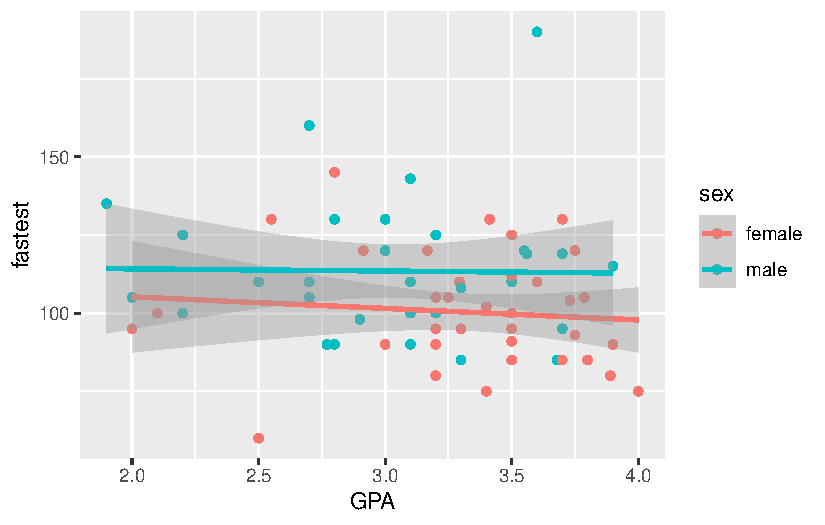
\includegraphics{05-visualisierung_files/figure-pdf/unnamed-chunk-6-1.pdf}

}

\end{figure}

Wir sehen: Frauen haben tendenziell langsamere Höchstgeschwindigkeiten
als Männer, aber auch hier überlappen sich die Balken.

Ein weiterer wichtiger Diagrammtyp ist das \emph{Histogramm}. Es gibt
an, wie oft ein bestimmtes ``Level'' einer Variable in den Daten
vorkommt, zum Beispiel wie folgt:

\begin{Shaded}
\begin{Highlighting}[]
\NormalTok{m111survey }\SpecialCharTok{\%\textgreater{}\%} 
  \FunctionTok{ggplot}\NormalTok{(}\FunctionTok{aes}\NormalTok{(}\AttributeTok{x =}\NormalTok{ fastest)) }\SpecialCharTok{+}
  \FunctionTok{geom\_histogram}\NormalTok{(}\AttributeTok{fill =} \StringTok{"burlywood"}\NormalTok{, }\AttributeTok{color =} \StringTok{"black"}\NormalTok{)}
\end{Highlighting}
\end{Shaded}

\begin{verbatim}
`stat_bin()` using `bins = 30`. Pick better value with `binwidth`.
\end{verbatim}

\begin{figure}[H]

{\centering 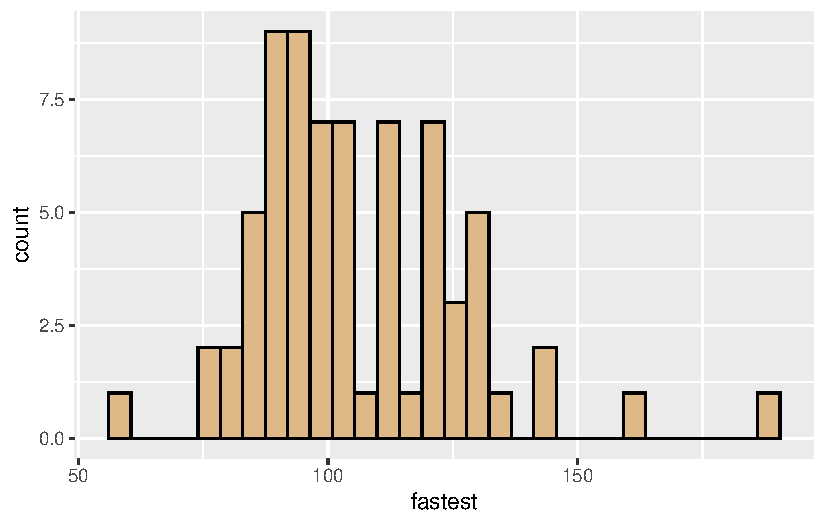
\includegraphics{05-visualisierung_files/figure-pdf/unnamed-chunk-7-1.pdf}

}

\end{figure}

Ähnliches kann durch das Layer \texttt{geom\_density()} erreicht werden.
Dieses gibt nicht die Anzahl, sondern die Verteilung der
Geschwindigkeiten an.

\begin{Shaded}
\begin{Highlighting}[]
\NormalTok{m111survey }\SpecialCharTok{\%\textgreater{}\%} 
  \FunctionTok{ggplot}\NormalTok{(}\FunctionTok{aes}\NormalTok{(}\AttributeTok{x =}\NormalTok{ fastest)) }\SpecialCharTok{+}
  \FunctionTok{geom\_density}\NormalTok{(}\AttributeTok{fill =} \StringTok{"burlywood"}\NormalTok{)}
\end{Highlighting}
\end{Shaded}

\begin{figure}[H]

{\centering 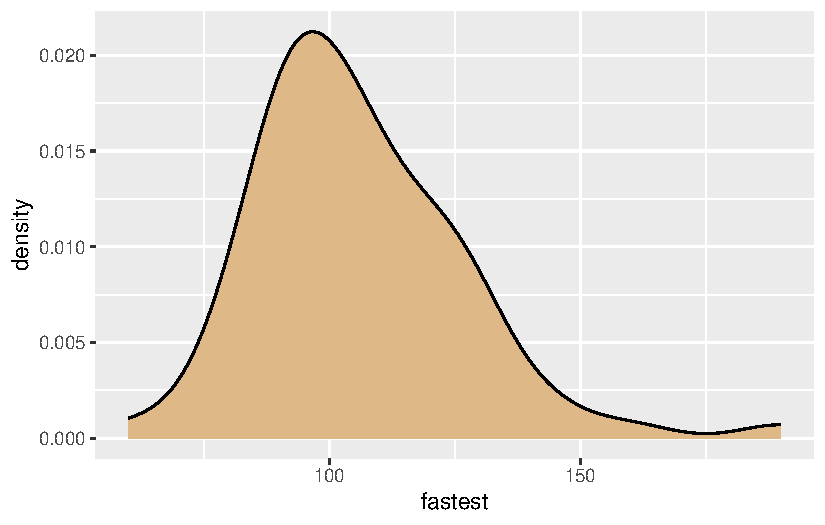
\includegraphics{05-visualisierung_files/figure-pdf/unnamed-chunk-8-1.pdf}

}

\end{figure}

\hypertarget{erweiterungen}{%
\subsection{Erweiterungen}\label{erweiterungen}}

\hypertarget{themes}{%
\subsubsection{Themes}\label{themes}}

Themes bestimmen das Aussehen unseres Diagramms, vor allem den
Hintergrund und die Markierungen. Standardmäßig haben Diagramme einen
grauen Hintergrund mit weißen Gitternetzlinien. Nutzen wir bei unserem
Histogramm \texttt{theme\_minimal()} als Theme, sieht das folgendermaßen
aus:

\begin{Shaded}
\begin{Highlighting}[]
\NormalTok{m111survey }\SpecialCharTok{\%\textgreater{}\%} 
  \FunctionTok{ggplot}\NormalTok{(}\FunctionTok{aes}\NormalTok{(}\AttributeTok{x =}\NormalTok{ fastest)) }\SpecialCharTok{+}
  \FunctionTok{geom\_histogram}\NormalTok{(}\AttributeTok{fill =} \StringTok{"burlywood"}\NormalTok{, }\AttributeTok{color =} \StringTok{"black"}\NormalTok{) }\SpecialCharTok{+}
  \FunctionTok{theme\_minimal}\NormalTok{()}
\end{Highlighting}
\end{Shaded}

\begin{verbatim}
`stat_bin()` using `bins = 30`. Pick better value with `binwidth`.
\end{verbatim}

\begin{figure}[H]

{\centering 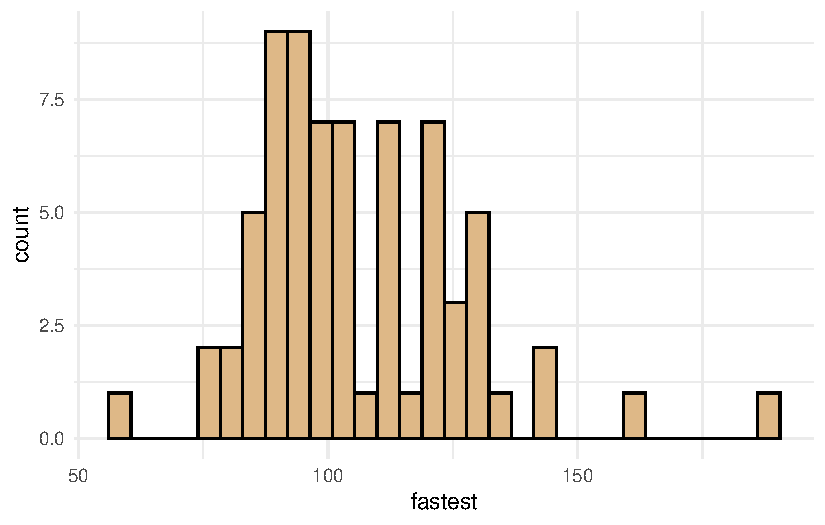
\includegraphics{05-visualisierung_files/figure-pdf/unnamed-chunk-9-1.pdf}

}

\end{figure}

Das gleiche Diagramm mit dem \texttt{theme\_bw()} sieht so aus:

\begin{Shaded}
\begin{Highlighting}[]
\NormalTok{m111survey }\SpecialCharTok{\%\textgreater{}\%} 
  \FunctionTok{ggplot}\NormalTok{(}\FunctionTok{aes}\NormalTok{(}\AttributeTok{x =}\NormalTok{ fastest)) }\SpecialCharTok{+}
  \FunctionTok{geom\_histogram}\NormalTok{(}\AttributeTok{fill =} \StringTok{"burlywood"}\NormalTok{, }\AttributeTok{color =} \StringTok{"black"}\NormalTok{) }\SpecialCharTok{+}
  \FunctionTok{theme\_bw}\NormalTok{()}
\end{Highlighting}
\end{Shaded}

\begin{verbatim}
`stat_bin()` using `bins = 30`. Pick better value with `binwidth`.
\end{verbatim}

\begin{figure}[H]

{\centering 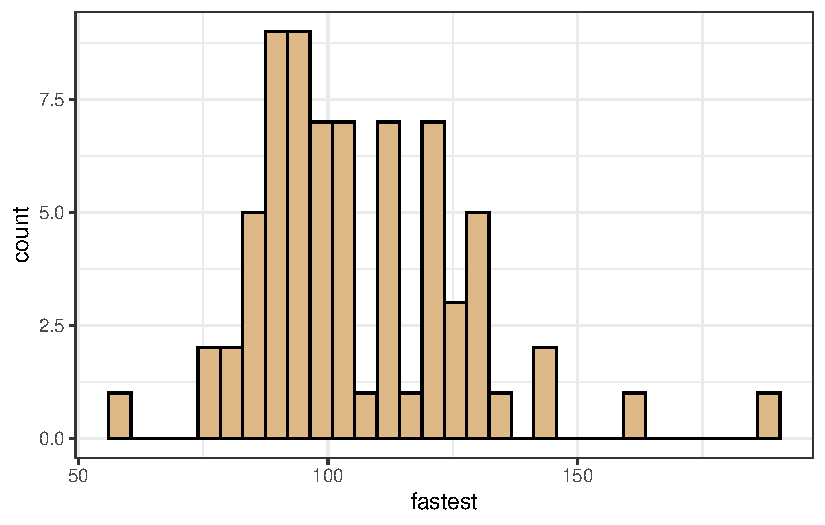
\includegraphics{05-visualisierung_files/figure-pdf/unnamed-chunk-10-1.pdf}

}

\end{figure}

Es gibt noch zahlreiche weitere Themes, die man mit
\texttt{theme\_...()} auswählen kann.

\hypertarget{titel-und-beschriftungen}{%
\subsubsection{Titel und
Beschriftungen}\label{titel-und-beschriftungen}}

So, wie die Diagramme jetzt aussehen, sind sie etwas kahl. Wenn wir sie
später irgendwo benutzen wollen, sollten wir sie so formatieren, dass
man ihnen den Sinn entnehmen kann. Das können wir mithilfe von Titeln
und Beschriftungen erreichen.

Um einen Titel hinzuzufügen, gibt es das Layer \texttt{ggtitle()}. Es
wird folgendermaßen verwendet:

\begin{Shaded}
\begin{Highlighting}[]
\NormalTok{m111survey }\SpecialCharTok{\%\textgreater{}\%} 
  \FunctionTok{ggplot}\NormalTok{(}\FunctionTok{aes}\NormalTok{(}\AttributeTok{x =}\NormalTok{ fastest)) }\SpecialCharTok{+}
  \FunctionTok{geom\_histogram}\NormalTok{(}\AttributeTok{fill =} \StringTok{"burlywood"}\NormalTok{, }\AttributeTok{color =} \StringTok{"black"}\NormalTok{) }\SpecialCharTok{+}
  \FunctionTok{theme\_bw}\NormalTok{() }\SpecialCharTok{+}
  \FunctionTok{ggtitle}\NormalTok{(}\StringTok{"Höchste je gefahrene Geschwindigkeit"}\NormalTok{,}
          \StringTok{"Daten aus einer Befragung unter Studenten des Georgetown College in Kentucky"}\NormalTok{)}
\end{Highlighting}
\end{Shaded}

\begin{verbatim}
`stat_bin()` using `bins = 30`. Pick better value with `binwidth`.
\end{verbatim}

\begin{figure}[H]

{\centering 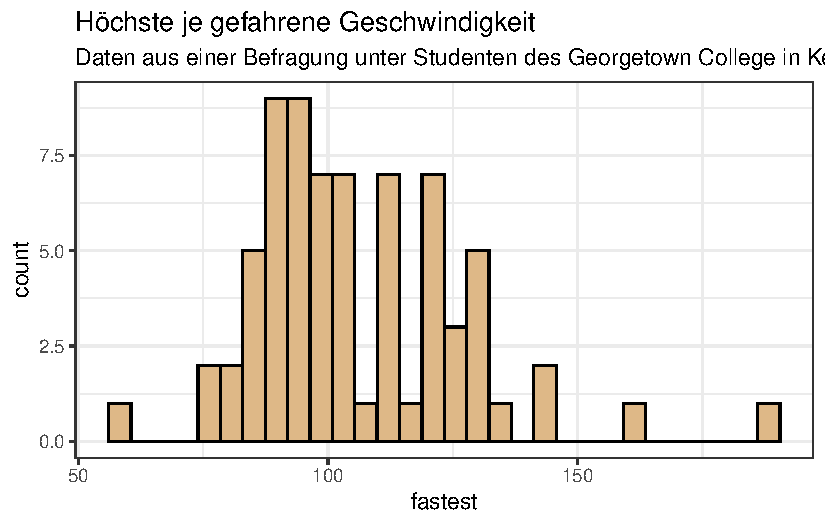
\includegraphics{05-visualisierung_files/figure-pdf/unnamed-chunk-11-1.pdf}

}

\end{figure}

Nun sind die Achsenbeschriftungen aber auch noch auf Englisch und nicht
sehr deskriptiv. Wir können sie mithilfe von \texttt{xlab()} und
\texttt{ylab()} ändern:

\begin{Shaded}
\begin{Highlighting}[]
\NormalTok{m111survey }\SpecialCharTok{\%\textgreater{}\%} 
  \FunctionTok{ggplot}\NormalTok{(}\FunctionTok{aes}\NormalTok{(}\AttributeTok{x =}\NormalTok{ fastest)) }\SpecialCharTok{+}
  \FunctionTok{geom\_histogram}\NormalTok{(}\AttributeTok{fill =} \StringTok{"burlywood"}\NormalTok{, }\AttributeTok{color =} \StringTok{"black"}\NormalTok{) }\SpecialCharTok{+}
  \FunctionTok{theme\_bw}\NormalTok{() }\SpecialCharTok{+}
  \FunctionTok{ggtitle}\NormalTok{(}\StringTok{"Höchste je gefahrene Geschwindigkeit"}\NormalTok{,}
          \StringTok{"Daten aus einer Befragung unter Studenten des Georgetown College in Kentucky"}\NormalTok{) }\SpecialCharTok{+}
  \FunctionTok{xlab}\NormalTok{(}\StringTok{"Geschwindigkeit in Meilen pro Stunde"}\NormalTok{) }\SpecialCharTok{+}
  \FunctionTok{ylab}\NormalTok{(}\StringTok{"Anzahl an Angaben"}\NormalTok{)}
\end{Highlighting}
\end{Shaded}

\begin{verbatim}
`stat_bin()` using `bins = 30`. Pick better value with `binwidth`.
\end{verbatim}

\begin{figure}[H]

{\centering 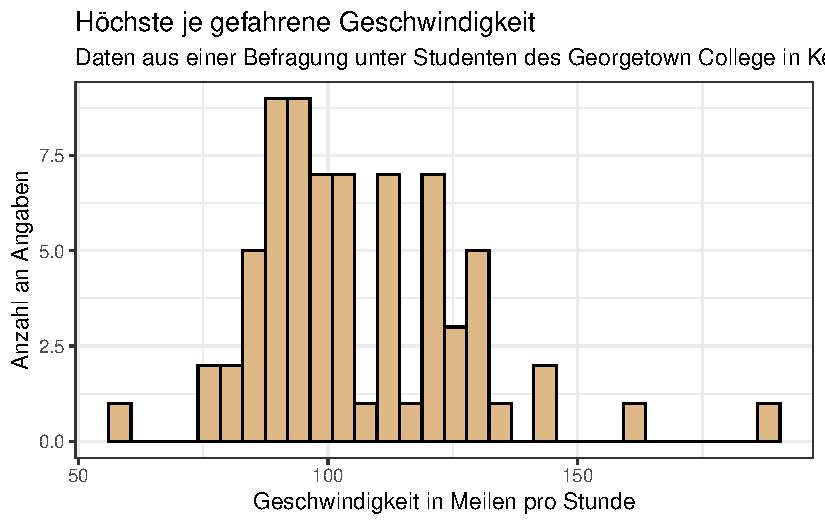
\includegraphics{05-visualisierung_files/figure-pdf/unnamed-chunk-12-1.pdf}

}

\end{figure}

Wie wir in der Ausgabe sehen, sollte man auch noch die Breite der Säulen
festlegen. Das sollte immer im Kontext der Daten erfolgen: Eine
Säulenbreite von 50 würde die Daten unzureichend darstellen, während
eine Säulenbreite von 1 zu fein ist (eventuell mehrmals nur eine Angabe
pro Säule). Eine Säulenbreite von 5 ist wahrscheinlich angemessen:

\begin{Shaded}
\begin{Highlighting}[]
\NormalTok{m111survey }\SpecialCharTok{\%\textgreater{}\%} 
  \FunctionTok{ggplot}\NormalTok{(}\FunctionTok{aes}\NormalTok{(}\AttributeTok{x =}\NormalTok{ fastest)) }\SpecialCharTok{+}
  \FunctionTok{geom\_histogram}\NormalTok{(}\AttributeTok{fill =} \StringTok{"burlywood"}\NormalTok{, }\AttributeTok{color =} \StringTok{"black"}\NormalTok{, }\AttributeTok{binwidth =} \DecValTok{5}\NormalTok{) }\SpecialCharTok{+}
  \FunctionTok{theme\_bw}\NormalTok{() }\SpecialCharTok{+}
  \FunctionTok{ggtitle}\NormalTok{(}\StringTok{"Höchste je gefahrene Geschwindigkeit"}\NormalTok{,}
          \StringTok{"Daten aus einer Befragung unter Studenten des Georgetown College in Kentucky"}\NormalTok{) }\SpecialCharTok{+}
  \FunctionTok{xlab}\NormalTok{(}\StringTok{"Geschwindigkeit in Meilen pro Stunde"}\NormalTok{) }\SpecialCharTok{+}
  \FunctionTok{ylab}\NormalTok{(}\StringTok{"Anzahl an Angaben"}\NormalTok{)}
\end{Highlighting}
\end{Shaded}

\begin{figure}[H]

{\centering 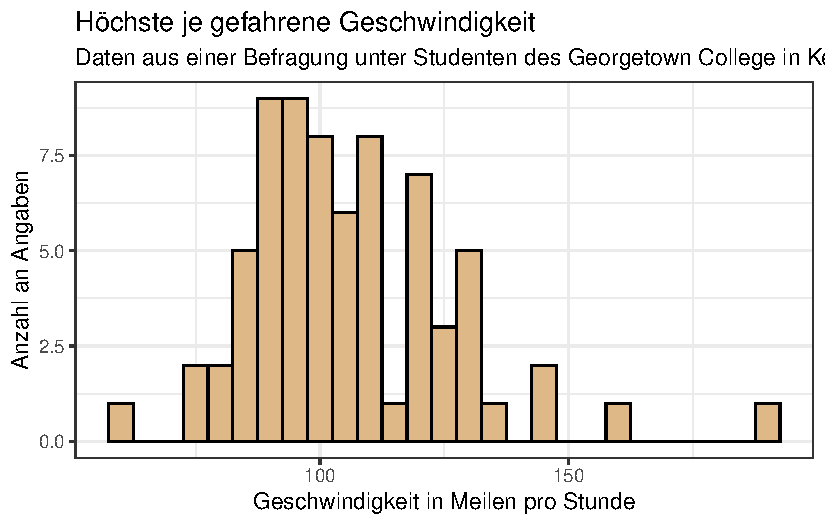
\includegraphics{05-visualisierung_files/figure-pdf/unnamed-chunk-13-1.pdf}

}

\end{figure}

\hypertarget{achsenskalierung}{%
\subsubsection{Achsenskalierung}\label{achsenskalierung}}

Wir sehen im Diagramm oben, dass wir nur zwei x-Achsen-Markierungen
haben, bei 100 und 150 Meilen pro Stunde. Das ist aber relativ wenig.
Wir können mehr Markierungen hinzufügen, indem wir festlegen, wo sie zu
sehen sein sollen. Ebenso ist unschön, dass wir auf der y-Achse keine
ganzen Zahlen haben, obwohl wir nur zählen, wie häufig (ganze Zahlen)
die angegebene Geschwindigkeit genannt wird. Auch hier ändern wir die
Skala:

\begin{Shaded}
\begin{Highlighting}[]
\NormalTok{m111survey }\SpecialCharTok{\%\textgreater{}\%} 
  \FunctionTok{ggplot}\NormalTok{(}\FunctionTok{aes}\NormalTok{(}\AttributeTok{x =}\NormalTok{ fastest)) }\SpecialCharTok{+}
  \FunctionTok{geom\_histogram}\NormalTok{(}\AttributeTok{fill =} \StringTok{"burlywood"}\NormalTok{, }\AttributeTok{color =} \StringTok{"black"}\NormalTok{, }\AttributeTok{binwidth =} \DecValTok{5}\NormalTok{) }\SpecialCharTok{+}
  \FunctionTok{theme\_bw}\NormalTok{() }\SpecialCharTok{+}
  \FunctionTok{ggtitle}\NormalTok{(}\StringTok{"Höchste je gefahrene Geschwindigkeit"}\NormalTok{,}
          \StringTok{"Daten aus einer Befragung unter Studenten des Georgetown College in Kentucky"}\NormalTok{) }\SpecialCharTok{+}
  \FunctionTok{xlab}\NormalTok{(}\StringTok{"Geschwindigkeit in Meilen pro Stunde"}\NormalTok{) }\SpecialCharTok{+}
  \FunctionTok{ylab}\NormalTok{(}\StringTok{"Anzahl an Angaben"}\NormalTok{) }\SpecialCharTok{+}
  \FunctionTok{scale\_x\_continuous}\NormalTok{(}\AttributeTok{breaks =} \FunctionTok{c}\NormalTok{(}\DecValTok{75}\NormalTok{, }\DecValTok{100}\NormalTok{, }\DecValTok{125}\NormalTok{, }\DecValTok{150}\NormalTok{, }\DecValTok{175}\NormalTok{)) }\SpecialCharTok{+}
  \FunctionTok{scale\_y\_continuous}\NormalTok{(}\AttributeTok{breaks =} \FunctionTok{c}\NormalTok{(}\DecValTok{0}\NormalTok{, }\DecValTok{2}\NormalTok{, }\DecValTok{4}\NormalTok{, }\DecValTok{6}\NormalTok{, }\DecValTok{8}\NormalTok{))}
\end{Highlighting}
\end{Shaded}

\begin{figure}[H]

{\centering 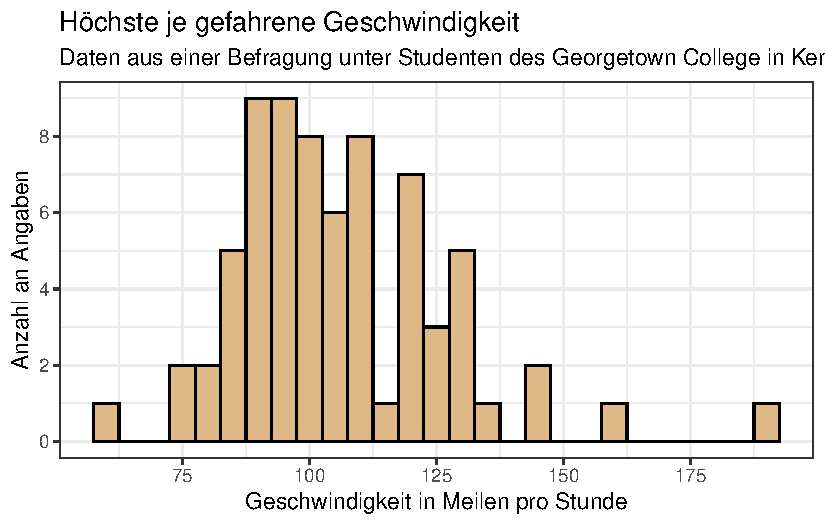
\includegraphics{05-visualisierung_files/figure-pdf/unnamed-chunk-14-1.pdf}

}

\end{figure}

\hypertarget{weitere-ressourcen}{%
\subsection{Weitere Ressourcen}\label{weitere-ressourcen}}

Welche Mittel man für ein schönes Diagramm braucht, hängt sehr davon ab,
welche Art von Daten man hat und was man darstellen möchte. In vielen
Fällen ist es das Einfachste, nach den Layern zu googeln, die man
benutzen will. Hier sind noch einige weitere Ressourcen, in denen man
nachschlagen kann:

\begin{itemize}
\item
  Das \texttt{ggplot2}-Cheat Sheet:
  \href{https://www.maths.usyd.edu.au/u/UG/SM/STAT3022/r/current/Misc/data-visualization-2.1.pdf}{LINK}
\item
  Die \texttt{ggplot2}-Dokumentation:
  \href{https://ggplot2.tidyverse.org/reference/}{LINK}
\item
  Eine weitergehende Zusammenfassung der Uni Göttingen:
  \href{https://md.psych.bio.uni-goettingen.de/mv/unit/ggplot2/ggplot2.html}{LINK}
\end{itemize}



\end{document}
